\begin{frame}[fragile]{\textit{Methodology} --- Grid Index for a Single Team}
%% Some methodology, mostly to motivate the usage the grid index as an easily to understand and CONFIGURABLE index data structure
%% The figure also introduces the general procedure of a secondary approach, and teases trade-offs
%% It should become clear, how the parameters induce interesting trade-offs, which govern how effective index intersection can become
%% Procedure:
%  \item[1)] For all indices: Map the query rectangle to relevant "leafs"
%  \item[2)] Optimise the ``query'' plan
%  \item[3a)] Fetch relevant leafs
%  \item[3b)] Combine leafs/index intersection
%  \item[4)] Fetch actual candidate rows
%% Key points: grid index, procedure, trade-offs (treaser), configurability and parameters

% Uncomment the following block to restore the original, animated grid-index draft.
\begin{columns}
\column{0.4\textwidth}
% \centering
% {\scriptsize Data Space}
\only<1>{
  \begin{figure}
      \centering
      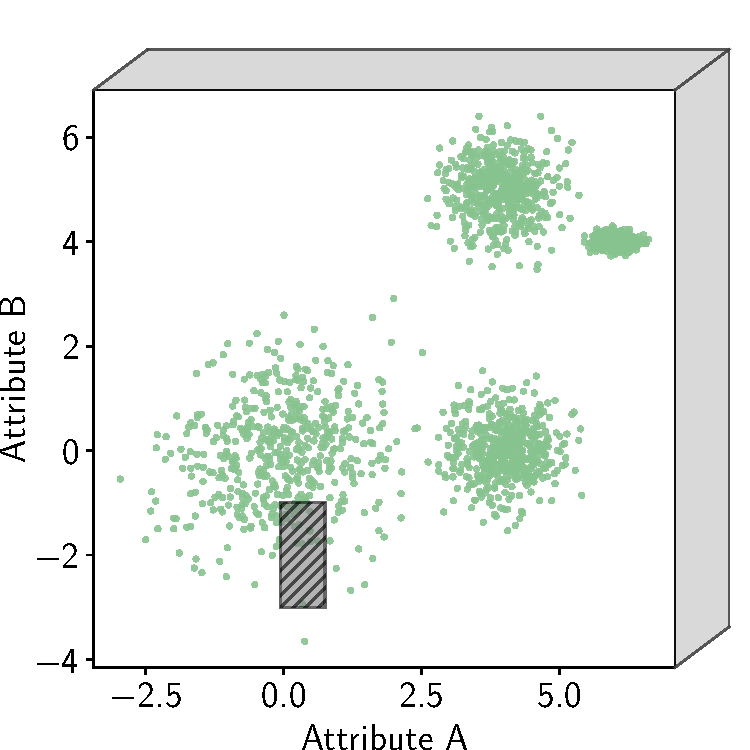
\includegraphics[width=\textwidth]{figures/grid_index_plain}
  \end{figure}
}
\only<2-3>{
    \begin{figure}
        \centering
        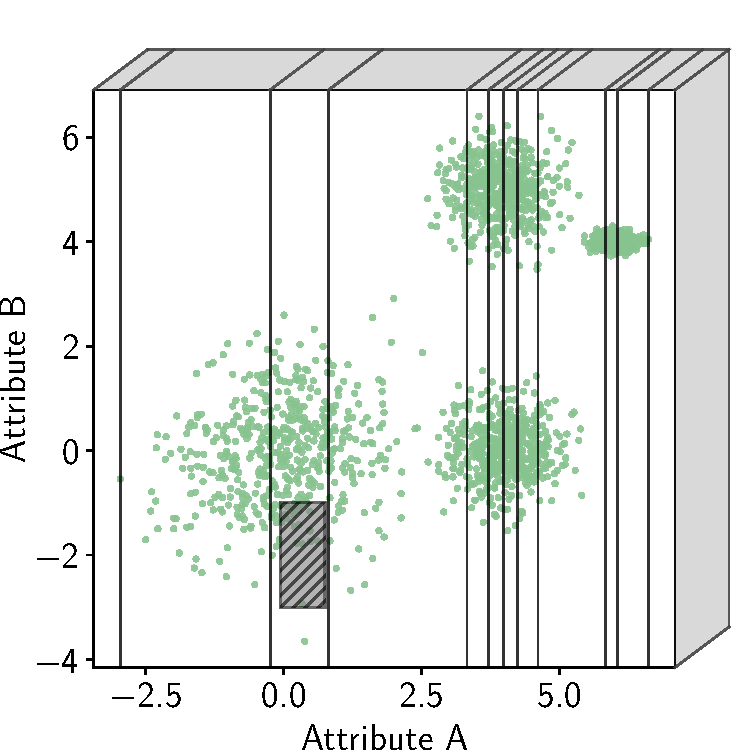
\includegraphics[width=\textwidth]{figures/grid_index_1D}
    \end{figure}
}
\only<4>{
    \begin{figure}
        \centering
        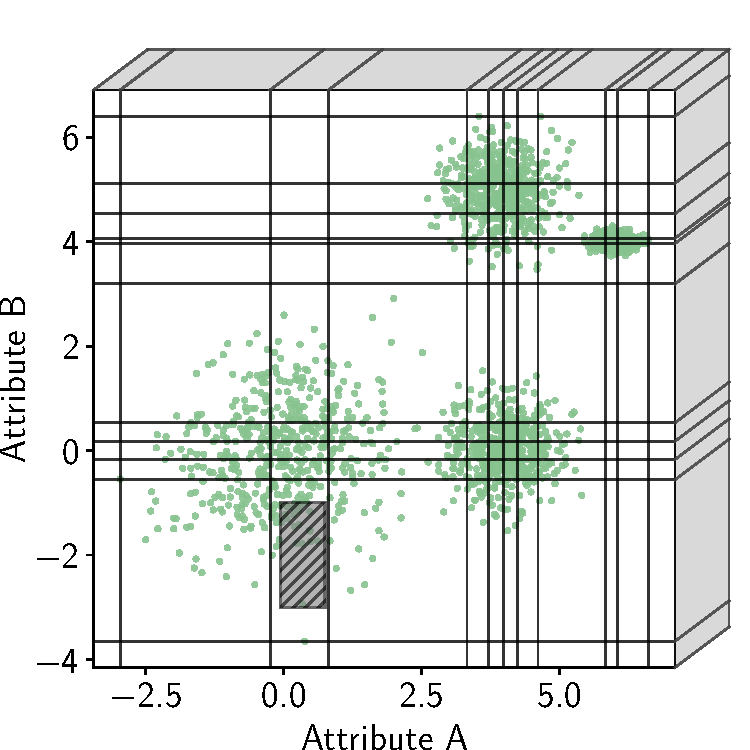
\includegraphics[width=\textwidth]{figures/grid_index_2D}
    \end{figure}
}
\only<5->{
    \begin{figure}
        \centering
        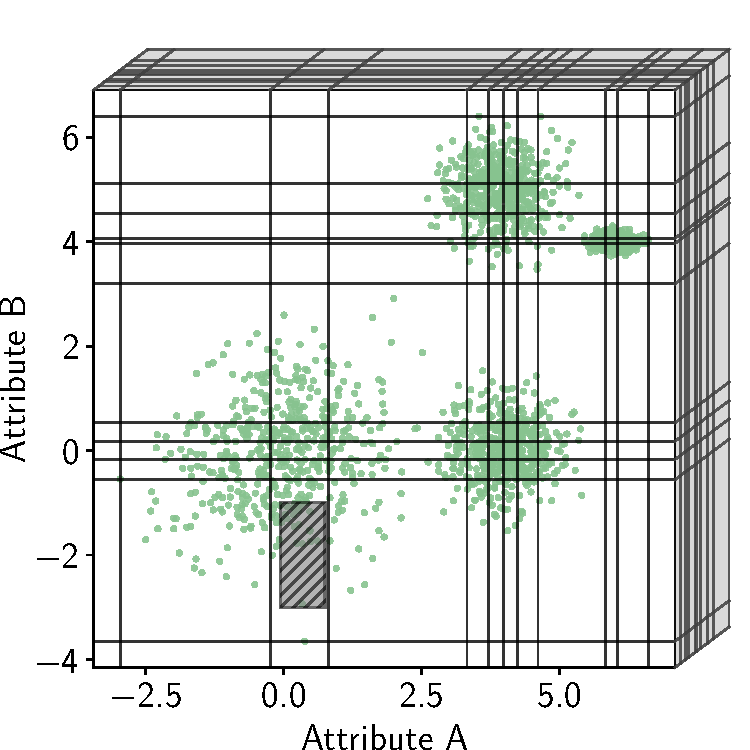
\includegraphics[width=\textwidth]{figures/grid_index_3D}
    \end{figure}
}
\column{0.6\textwidth}
\uncover<2->{
  \begin{tikzpicture}[x=1mm,y=1mm]
    \def\gshift{1.4}%
    \def\goffset{5}%
    \def\goffsetY{14}%
    \def\cellsize{4.5}%
    \def\npages{7}
    \def\pw{9}
    \def\ph{6}
    \def\headerh{3}
    \def\payloady{1}
    \def\payloadh{\ph-\headerh-1}
    \newcommand{\LeafGrid}[7]{%
      \begin{scope}[shift={({#6},{#7})}]
        \pgfmathtruncatemacro{\R}{#2}
        \pgfmathtruncatemacro{\C}{#3}
        \foreach \r in {1,...,\R}{
          \foreach \c in {1,...,\C}{
            \pgfmathsetmacro{\x}{(\c-1)*#4}
            \pgfmathsetmacro{\y}{(\R-\r)*#5}
            \node[gridcell] (#1-r\r-c\c) at (\x,\y) {$\cdot$};
          }
        }
      \end{scope}%
    }
    % Cheaper stand-in for \LeafGrid: only draws the top row and right column
    % (the "rim") of the grid. Used for back layers of the 3D stack that are
    % almost entirely occluded by the layers in front of them, so drawing the
    % full R x C grid of nodes would be wasted rendering time.
    \newcommand{\LeafGridRim}[7]{%
      \begin{scope}[shift={({#6},{#7})}]
        \pgfmathtruncatemacro{\R}{#2}
        \pgfmathtruncatemacro{\C}{#3}
        \foreach \c in {1,...,\C}{
          \pgfmathsetmacro{\x}{(\c-1)*#4}
          \pgfmathsetmacro{\y}{(\R-1)*#5}
          \node[gridcell] (#1-r1-c\c) at (\x,\y) {$\cdot$};
        }
        \foreach \r in {2,...,\R}{
          \pgfmathsetmacro{\x}{(\C-1)*#4}
          \pgfmathsetmacro{\y}{(\R-\r)*#5}
          \node[gridcell] (#1-r\r-c\C) at (\x,\y) {$\cdot$};
        }
      \end{scope}%
    }
    \pgfmathtruncatemacro{\N}{\npages}
    \foreach \i in {1,...,\N} {
        \pgfmathsetmacro{\x}{(\i-1)*\pw}
        \draw (\x,0) rectangle ++(\pw,\ph);
        \ifdim \headerh pt>0pt
        \fill[black!8] (\x,\ph-\headerh) rectangle ++(\pw,\headerh);
        \node[font=\scriptsize\bfseries] at (\x+0.5*\pw,\ph-0.5*\headerh) {Page \i};
        \fi
    }

    \node[text=black, font=\bfseries] at (-4.5,14.3) {Grid:};
    \node[text=black, font=\bfseries] at (-6,\ph/2.0) {SSD:};
    \node[text=black, font=\bfseries] at ({(\N+0.5)*\pw},\ph/2.0) {\ldots};

    \newcommand{\TapeSegment}[3]{%
        \pgfmathsetmacro{\start}{#2-1}
        \pgfmathsetmacro{\L}{#3}
        \pgfmathsetmacro{\nfull}{floor(\L)}
        \pgfmathsetmacro{\rem}{\L-\nfull}
        \foreach \k in {0,...,\nfull} {
        \ifnum \k<\nfull
            \pgfmathsetmacro{\xx}{(\start+\k)*\pw}
            \fill[#1] (\xx,\payloady) rectangle ++(\pw,\payloadh);
        \fi
        }
        \ifdim \rem pt>0pt
        \pgfmathsetmacro{\xrem}{(\start+\nfull)*\pw}
        \pgfmathsetmacro{\wrem}{\rem*\pw}
        \fill[#1] (\xrem,\payloady) rectangle ++(\wrem,\payloadh);
        \fi
    }
    \uncover<5->{
      % Back layers are almost fully covered by the layers drawn in front of
      % them, so only their top-row/right-column rim needs to be rendered.
      \foreach \shift in {9,8,...,3} {
        \pgfmathsetmacro{\offset}{\goffset + \shift*\gshift}
        \pgfmathsetmacro{\offsetY}{\goffsetY + \shift*\gshift}
        \LeafGridRim{arr1}{10}{10}{\cellsize}{\cellsize}{\offset}{\offsetY}
      }
      % The front two layers are fully visible, so draw them completely.
      \foreach \shift in {2,1} {
        \pgfmathsetmacro{\offset}{\goffset + \shift*\gshift}
        \pgfmathsetmacro{\offsetY}{\goffsetY + \shift*\gshift}
        \LeafGrid{arr1}{10}{10}{\cellsize}{\cellsize}{\offset}{\offsetY}
      }
    }
    \uncover<4->{\LeafGrid{arr1}{9}{10}{\cellsize}{\cellsize}{\goffset}{\goffsetY+\cellsize}}
    \LeafGrid{arr1}{1}{10}{\cellsize}{\cellsize}{\goffset}{\goffsetY}
    \coordinate (refcellcoord) at (\goffset+\cellsize, \goffsetY);
    \only<2>{
      \TapeSegment{\pagecolor}{1}{3.6}
      \TapeSegment{\pagecolor}{5}{2.8}
      \node[gridcell,fill=\pagecolor] (refcell) at (refcellcoord) {$\cdot$};
    }
    \uncover<3->{
      \node[gridcell,fill=color5] (refcell) at (refcellcoord) {$\cdot$};
    }
    \only<3>{
      \TapeSegment{\pagecolor}{1}{3.6}
      \TapeSegment{color5}{5}{2.8}
      \draw[halo arrow] (refcellcoord) to[out=60,in=40,looseness=0.95] ($(refcellcoord)+(30,-8)$);
    }
    \only<4>{
      \TapeSegment{\pagecolor}{1}{1.6}
      \TapeSegment{color5}{3}{0.8}
      \draw[halo arrow] (refcellcoord) to[out=50,in=50,looseness=0.95] ($(refcellcoord)+(13,-8)$);
      \TapeSegment{\pagecolor}{4}{1.8}
      \TapeSegment{\pagecolor}{6}{1.15}
    }
    \only<5->{
      \TapeSegment{\pagecolor}{1}{0.6}
      \TapeSegment{color5}{2}{0.8}
      \draw[halo arrow] (refcellcoord) to[out=40,in=60,looseness=0.95] ($(refcellcoord)+(5.2,-8)$);
      \TapeSegment{\pagecolor}{3}{0.1}
      \TapeSegment{\pagecolor}{4}{.2}
      \TapeSegment{\pagecolor}{5}{1.15}
      \TapeSegment{\pagecolor}{7}{.15}
    }
  \end{tikzpicture}
}
\end{columns}

\begin{tikzpicture}[remember picture,overlay]
  \only<2>{\node[overlay callout,draw,fill=color1!50,anchor=pointer,callout relative pointer={(210:0.8cm)}] at ($(current page text area.east)+(-2.2cm,-3.85cm)$) {\textbf{``Leaf''}};}
  \uncover<2-3>{\node[overlay callout,draw,fill=color2!60,anchor=pointer,callout relative pointer={(210:1.7cm)}] at ($(current page text area.north east)+(-4cm,-6cm)$) {$\mathbf{b^d=10^1}$ cells};}
  \only<4>{\node[overlay callout,draw,fill=color2!60,anchor=pointer,callout relative pointer={(210:1.7cm)}] at ($(current page text area.north east)+(-4cm,-6cm)$) {$\mathbf{b^d=10^2}$ cells};}
  \only<5>{\node[overlay callout,draw,fill=color2!60,anchor=pointer,callout relative pointer={(210:1.7cm)}] at ($(current page text area.north east)+(-4cm,-6cm)$) {$\mathbf{b^d=10^3}$ cells};}
  \uncover<3->{
    \draw[halo arrow] ($(current page text area.south west)+(1.9cm,1.8cm)$) to[out=40,in=160,looseness=0.95] ($(current page text area.south west)+(6cm,1.35cm)$);
    % \node[overlay callout,fill=color1!70,anchor=pointer,callout relative pointer={(220:1.3cm)}] at ($(current page text area.north east)+(-2cm,-7.3cm)$) {SSD};
  }
\end{tikzpicture}
\end{frame}
